% Instrucciones:
% > El archivo 'CIMATpreamble.sty' se require para crear la portada de la tesis.
% > La información de la portada de la tesis se puede personalizar en este documento
%   en las funciones agregadas por la descripción "portada"
% 

% LaTeX references (technical issues, workarounds)
% https://www.overleaf.com/learn/latex/Management_in_a_large_project ('including files' section)
% https://tex.stackexchange.com/questions/64839/how-to-change-listing-caption
% https://stackoverflow.com/questions/2709898/change-list-of-listings-text
% https://tex.stackexchange.com/questions/664/why-should-i-use-usepackaget1fontenc

%--------------------------------------------------------------------------------%
\documentclass[letterpaper,12pt,twoside]{book}         % clase y tamaño de fuente
\usepackage[spanish,es-nodecimaldot,es-tabla]{babel}   % language/hyphenation


% A continuación  se incluyen las librerias requeridas --------------------------%
\usepackage[Sonny]{fncychap}              % diseño de las páginas de la tesis
\usepackage{lipsum}                       % para crear texto en este formato
\usepackage[utf8]{inputenc}               % input encoding
\usepackage{graphicx}                     % libreria requerida por CIMATpreamble
\usepackage[svgnames,table]{xcolor}       % libreria requerida por CIMATpreamble
\usepackage{CIMATpreamble}                % diseño del gráfico de portada de CIMAT
\usepackage{tcolorbox}                    % caja que se usa en las palabras clave 
\usepackage{eso-pic}                      % para introducir la imagen del acta
%\usepackage{mi_preambulo}                % custom preamble
\usepackage{amsmath,amsfonts,amsthm}      % math packages
\usepackage{amsbsy}                       % bold symbols
\usepackage{amssymb}                      % math symbols
\usepackage{verbatim}                     % typewriter font enviroment
\usepackage{subcaption}                   % para usar con subfigures
\usepackage{float}                        % to position figures
\usepackage{enumerate}                    % listing items
\usepackage{listing}
\usepackage{caption}                      % custom caption
\usepackage{setspace}
\usepackage{url}                          % for url's
\usepackage{booktabs}                     % heavier lines in tables: bottom-rule

% bibliography
\usepackage[natbibapa]{apacite}           % APA Style Bibliography with natbib
\usepackage[nottoc]{tocbibind}            % bibliography is indexed but not numbered

\usepackage{emptypage} % libreria para que \cleardoublepage cree paginas sin formato
\makeatletter
\let\ps@firstpage\ps@empty
\makeatother

% Definición de colores  -----%
\definecolor{grisCIMAT}{RGB}{137,136,139}  % Color Instituional
\definecolor{rojoCIMAT}{RGB}{100,41,62}    % Color Instituional

\usepackage{hyperref}                      % Para incluir ligas
\hypersetup{                               % Asignación de colores para ligas
	colorlinks  =  true,             % Colours links instead of ugly boxes
	urlcolor    =  rojoCIMAT,        % Colour for external hyperlinks
	linkcolor   =  NavyBlue,         %customColorLink,  % Colour of internal links
	citecolor   =  Purple,           %FireBrick  % Colour for citations
}

%  Encabezados y pie de página
%\usepackage{fancyhdr}
\pagestyle{fancy}                          % Sets fancy header and footer
\fancyfoot{}                               % Delete current footer settings
\fancyhead[RE,LO]{}      %Page number in left on even pages and right on odd pages
\fancyhead[RO]{\nouppercase{\leftmark}}    % Chapter in the right on even pages
\fancyhead[LE]{\nouppercase{\rightmark}}   % Section in the left on odd pages
\renewcommand\headrulewidth{0.5pt}           % línea en el encabezado y grosor
\cfoot{\thepage }


%%% Mis comandos: -----------------------------%%%%%%%%%%%%%%%%%%%%%%%%%%%%%%%%%%%%
% Incluye tus nuevos comandos

\def\R{\mathbb{R}}                 % R para los núemros reales
\newcommand{\prob}{\mathbb{P}}     % P para denotar probabilidad

%--------------------------------------------------------------------------------%

% Por organización es deseable tener todas las figuras en un solo folder.
% Este comando indica cuál es para no tener que anotar toda la ruta para cada figura
\graphicspath{{figuras/}}


%% Portada:  ----------------------------------%%%%%%%%%%%%%%%%%%%%%%%%%%%%%%%%%%%%
% llena con la información de tu tesis 

\documentType{T E S I S}  % change to "T E S I N A" if it is the case
\title{El título de la tesis que puede ser de varios renglones \ldots}
\degree{Maestro en Ciencias}  
\degreeSecond{Probabilidad y Estadística} % opcional por si no hay orientación
\author{Nombre del estudiante}
\supervisor{Nombre del primer director}
\supervisorSecond{Nombre del segundo director}  % opcional si hay co-director
%Si no hay co-director, comentar o eliminar la linea anterior

\cityandyear{Guanajuato, Gto a XX de XX de XXXX}

%---------------------------------------------------------------------------------%

\begin{document}

\maketitle % Incluir portada
%\thispagestyle{empty} 

%% Acta de examen  ----------------------------%%%%%%%%%%%%%%%%%%%%%%%%%%%%%%%%%%%%
%  A añadir en la versión final una vez que se tenga 
\begingroup
 \thispagestyle{empty} 
 \AddToShipoutPicture*{
 \put(0,0){
		\parbox[b][\paperheight]{\paperwidth}{%
			\centering
			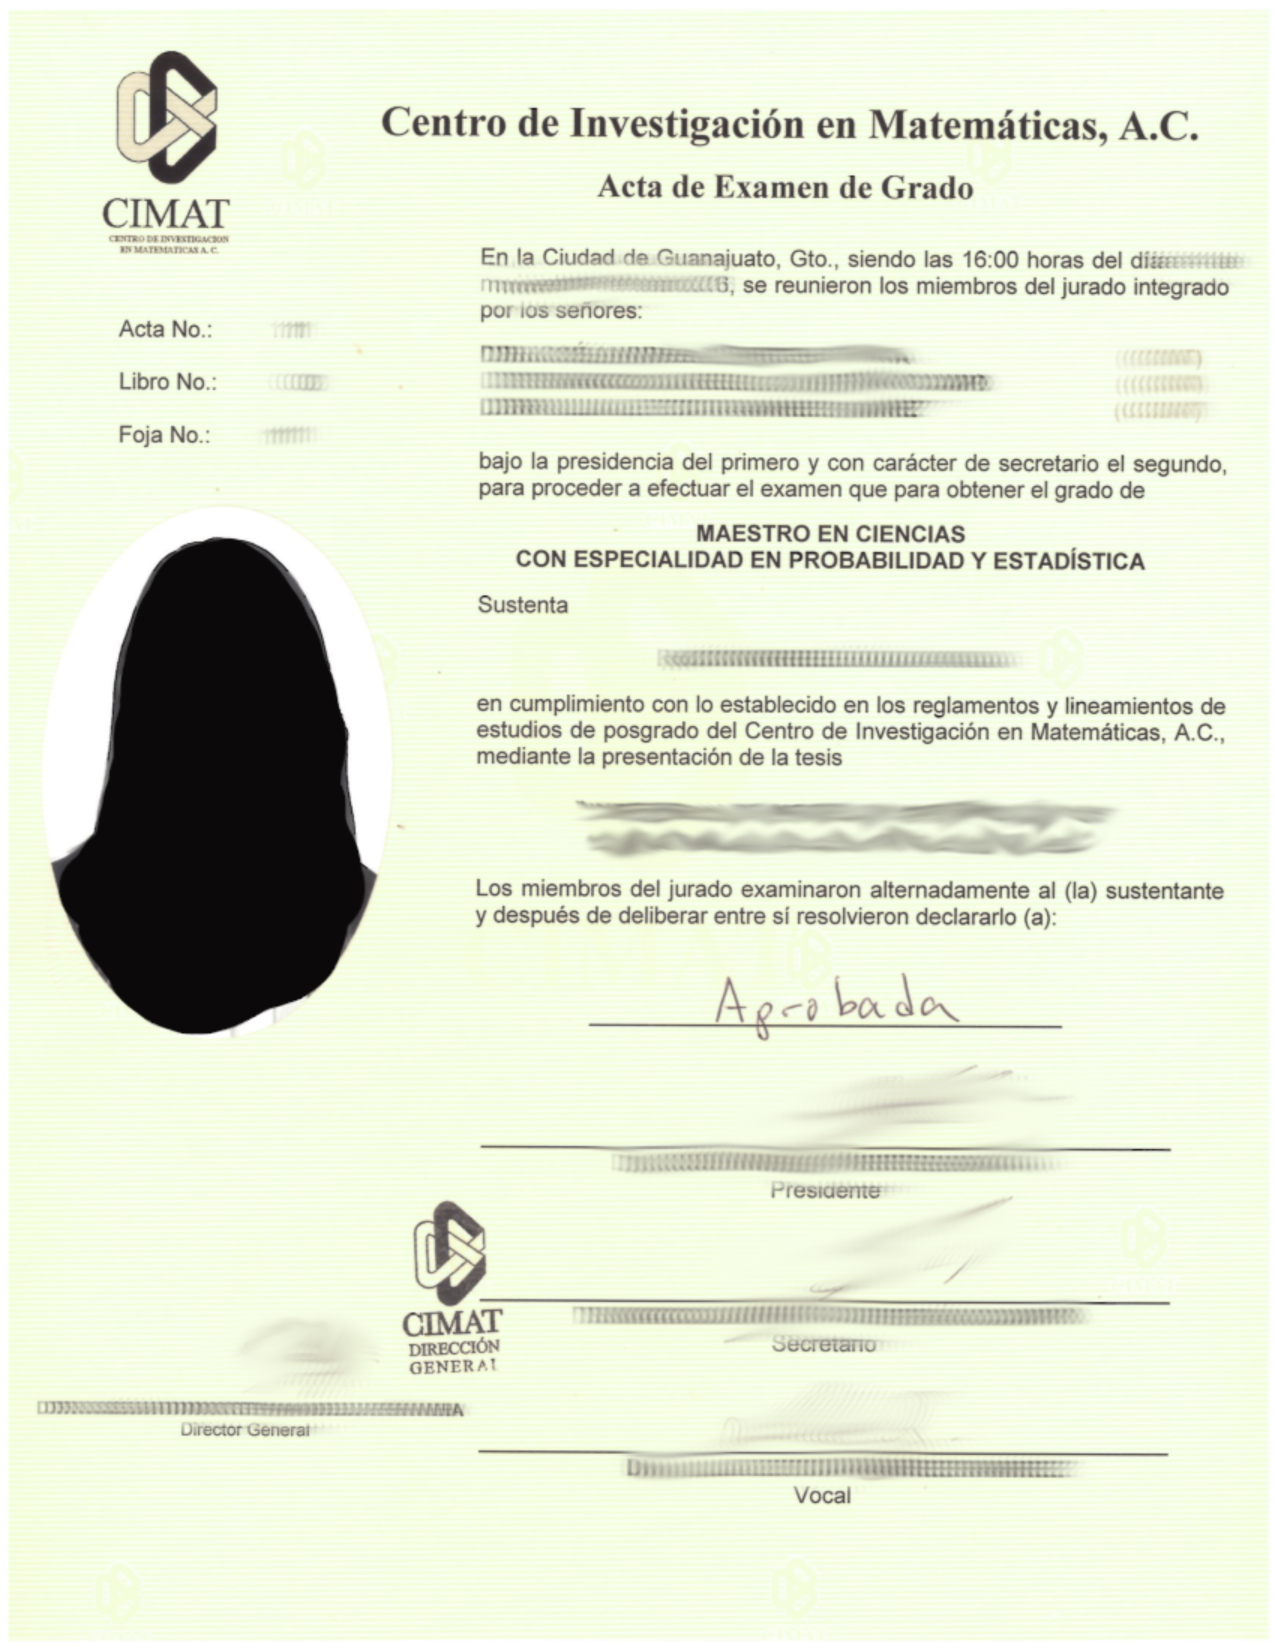
\includegraphics[scale=.97]{acta/Acta_Grado_Apellidos.pdf}            %
			\vfill
}}} 

\frontmatter

%% Dedicatoria  -------------------------------%%%%%%%%%%%%%%%%%%%%%%%%%%%%%%%%%%%%
\vspace*{\fill}
\begin{flushright}%
  \emph{Dedico esta tesis a estas personas tan importantes ...}
  \thispagestyle{empty}
\end{flushright}
\vspace*{\fill}
\cleardoublepage

%% Agradecimientos  ---------------------------%%%%%%%%%%%%%%%%%%%%%%%%%%%%%%%%%%%%
\phantomsection
% -*- coding: UTF-8; -*-


\chapter*{Agradecimientos} 
\label{Agradecimientos}
\addcontentsline{toc}{chapter}{Agradecimientos}

% Es requisitio de la tesis proporcionar, en la sección de agradecimientos de la tesis, los créditos 
% correspondientes por los apoyos recibidos del CONAHCyT o de la Institución que hubiese aportado cualquier 
% financiamiento para la realización de los estudios o de la tesis. [No aplica si el alumno no tuvo beca 
% CONAHCYT o de otro tipo en ninguno de sus semestres].

Gracias al Centro de Investigación en Matemáticas (CIMAT), por ... . Agradezco también al Consejo Nacional de Ciencia y Tecnología (CONACYT), por el apoyo económico con una beca de meatría etc..\bigskip 

Agradezco a mi asesor y ....\bigskip

Gracias a mis familia porque siempre ....\bigskip

También agradezco a ....


\cleardoublepage

%% Resumen ------------------------------------%%%%%%%%%%%%%%%%%%%%%%%%%%%%%%%%%%%%
\phantomsection
% -*- coding: UTF-8; -*-

\chapter*{Resumen} 
\label{chap:resumen}
\addcontentsline{toc}{chapter}{Resumen}

Este trabajo ...\lipsum[100]\lipsum[100]


\vspace{2cm}  %Añadir espacio vertical


\begin{tcolorbox}[colback=white!5,colframe=black!10!white,coltitle=white!10!black, fonttitle=\bfseries,title=Palabras Clave]
	Primera, Segunda, Tercera,..., Máximo 8.
\end{tcolorbox}

\cleardoublepage

%% Índice, lista de fituras y lista de tablas  %%%%%%%%%%%%%%%%%%%%%%%%%%%%%%%%%%%%

\phantomsection
\renewcommand\contentsname{Índice general}
\addcontentsline{toc}{chapter}{Índice general}
\tableofcontents
\cleardoublepage

\listoffigures
\cleardoublepage

\listoftables
\cleardoublepage

%% Incluir Capítulos y demas elementos  -------%%%%%%%%%%%%%%%%%%%%%%%%%%%%%%%%%%%%

\mainmatter
\spacing{1.5}  % Interlinieado para el resto del documento %

%% Introduccion y capitulos -------------------%

% -*- coding: UTF-8; -*-

\chapter{Introducción} 
\label{chap:intro}



El pbormema de ...las referencias que principalemnte se consideran son los trabajos de  \citet{Liu2008,Casella2002} y  \citep[como por ejemplo][entre otros]{Kotecha1999, Horrace2005}, donde  ... 

\lipsum[17]

\lipsum[2-4]

\lipsum[17]

\chapter{Título del Primer Capítulo}
\label{chap:Mod_Det}

\lipsum[10] Este es una referencia a un sitio web \url{https://www.cdc.gov/spanish/index.html}.

\section{Primera Sección}
\lipsum[100] 

\subsection{Nombre de subsección 2-1-1}
\lipsum[100] 

En la Figura \ref{fig:SEIR_sim0} se tiene...

\begin{figure}[h]
	\centering
	\includegraphics[width=9cm,keepaspectratio]{SEIR_sim0.pdf}
	\caption{Curvas epidémicas correspondientes a la simulación base.}
	\label{fig:SEIR_sim0}
\end{figure}

\lipsum[100]

\subsection{Nombre de subsección 2-1-2}
\lipsum[100]
 
 
La Tabla~\ref{tab:ejem} muestra...

\begin{table}[ht]
	\centering
	\caption{Estadísticas de la distribución}
	\label{tab:ejem}
	\resizebox{\textwidth}{!}{%
		\begin{tabular}{rrrrrrrrrr}
			\hline
			&$\beta_1$ &$\lambda_1$ & $\phi$ & $\omega$ & $\gamma$ & $\mu$ & $\beta_2$ & $\lambda_2$ & $\alpha$ \\
			\hline
			2.5\% & 0.1023 & 0.3568 & 0.0326 & 0.1767 & 0.1772 & 0.0358 & 0.3178 & 0.3635 & 441.03 \\ 
			50\% & 0.1406 & 0.4898 & 0.0454 & 0.2228 & 0.2423 & 0.0481 & 0.4125 & 0.5198 & 562.66 \\ 
			97.5\% & 0.1769 & 0.6412 & 0.2174 & 0.3198 & 0.3209 & 0.0639 & 0.5023 & 0.6426 & 598.59 \\ 
			Mean & 0.1403 & 0.4959 & 0.0647 & 0.2316 & 0.2484 & 0.0490 & 0.4117 & 0.5124 & 554.67\\
			\hline
		\end{tabular}
	}
\end{table}
\lipsum[100]

\section{Subsección 2}
\lipsum[100] 

\subsection{Nombre de subsección 2-2-1}
\lipsum[17] 

\subsection{Nombre de subsección 2-2-2}
\lipsum[10]
\lipsum[100]

\subsection{Nombre de subsección 2-2-3}
\lipsum[100]
   
   


\chapter{Título del tercer capítulo}
\label{chap:Infe}

\lipsum[10]


\section{Subsección 1}
\lipsum[100]. La Figura \ref{fig:subfiguras} presenta... La Figura \ref{fig:primera}... mientras que Figura \ref{fig:segunda}

\begin{figure}
	\centering
	\begin{subfigure}{0.45\textwidth}
		\includegraphics[width=\textwidth]{ejemplo-fig1.png}
		\caption{Descripción primera.}
		\label{fig:primera}
	\end{subfigure}
	\hfill
	\begin{subfigure}{0.45\textwidth}
		\center
		\includegraphics[width=0.7\textwidth]{ejemplo-fig3.pdf}
		\caption{Descripción segunda.}
		\label{fig:segunda}
	\end{subfigure}
	\hfill
	\caption{Ejemplo de dos figuras usando la función `subfigure' y el paquete `subcaption'.}
	\label{fig:subfiguras}
\end{figure}

\lipsum[1-4]






\subsection{Nombre de subsección 3-1-1}
\lipsum[100]
   \begin{table}
	\begin{center}
		\begin{tabular}{ c c  c   c c  c  c c c c c}
			%\hline 
			Evento & DIC & Eff & WAIC & logMLIK  & $\overline{CPO}$ & $\overline{PIT}$  \\ \hline \hline
			Semanas AR1 & 1938 & 117.3 & 1958 & -1052.5 &  0.020 &  0.500 \\
			D\'ias AR1 & 10567 & 188.7 & 10567 & -5389.3 &  0.068 & 0.524 \\
			Semanas RW & 1940 & 114.0 & 1964 &  -1047.4 &  0.014 & 0.369 \\
			D\'ias RW & 10575 & 175.5 & 10653 & -5382.7 & 0.068 & 0.524 \\
			\hline  
		\end{tabular}
	\end{center}
	\caption{Criterios para evaluación de modelos.}
	\label{tab:CriteriosTemporal}
\end{table}


\subsection{Nombre de subsección 3-1-2}
\lipsum[17]

\section{Subsección 2}
\lipsum[100] 






\chapter{Conclusiones y trabajo futuro}

\lipsum[100]

%% Bibliography  ------------------------------%

% APA style according to apacite package: see mypreamble.sty line 21
\bibliographystyle{apacite} 
%no se añade al nombre la extensión del archivo .bib 
\bibliography{referencias}  

%% Appendix  ----------------------------------%

\appendix
\chapter{Nombre del primer apéndice}
\label{app:MCMC}

\lipsum[10]


\lipsum[2-4]

 
\chapter{Nombre del primer apéndice}
\label{app:MCMC}

\lipsum[2-4]

 

\backmatter
\end{document}



